In statistics and probabilistic machine learning, we frequently encounter integrals that cannot be solved analytically. A common form is:
\begin{equation}
\label{eq:mc-int}
I(\varphi) = \int \varphi(x)f(x) dx
\end{equation}
where $f(x)$ is a probability density function and $\varphi(x)$ is some function of interest.
Such integrals typically require numerical approximation methods.
The Monte Carlo approach to integration is based on a fundamental insight: if we can sample from the probability distribution $f(x)$, we can approximate the integral via the sample average. The Monte Carlo estimator is therefore defined as:
\begin{equation}
\label{eq:mc-estimator}
\hat{\mu}_n = \frac{1}{n} \sum_{i=1}^n \varphi(X_i) \quad \text{where} \quad X_1, \ldots, X_n \overset{\text{i.i.d.}}{\sim} f
\end{equation}
Integrals of the form shown in \eqref{eq:mc-int} commonly represent expectations under posterior distributions, marginal likelihoods, or normalization constants. This becomes clearer through the following examples, with $X \sim f$:
\begin{align*}
\varphi(x) = x &\quad \Rightarrow \quad I(\varphi) = \mathbb{E}_f[X] \\
\varphi(x) = \mathbb{I}(x \leq \gamma) &\quad \Rightarrow \quad I(\varphi) = F_X(\gamma) \\
\varphi(x) = 1 &\quad \Rightarrow \quad I(\varphi) = \int f(x)dx
\end{align*}

\begin{example}
\label{ex:sin}
    Consider the integral $I = \int_0^{\pi} \sin(x)\,dx$. The exact value is $I = 2$.
    Suppose we only have access to uniformly distributed random variables on the $[0, 1)$ interval.
    We therefore use substitution to transform the domain to $[0,1)$: $I = \pi \int_0^1 \sin(\pi \cdot u) du \approx \pi \cdot n^{-1} \sum_{i = 1}^n \sin(\pi \cdot U_i)$, where $U_i \overset{i.i.d.}{\sim} \text{Unif}(0,1)$ for all $i = 1,...,n$.
    
    \begin{figure}[h]
    \centering
    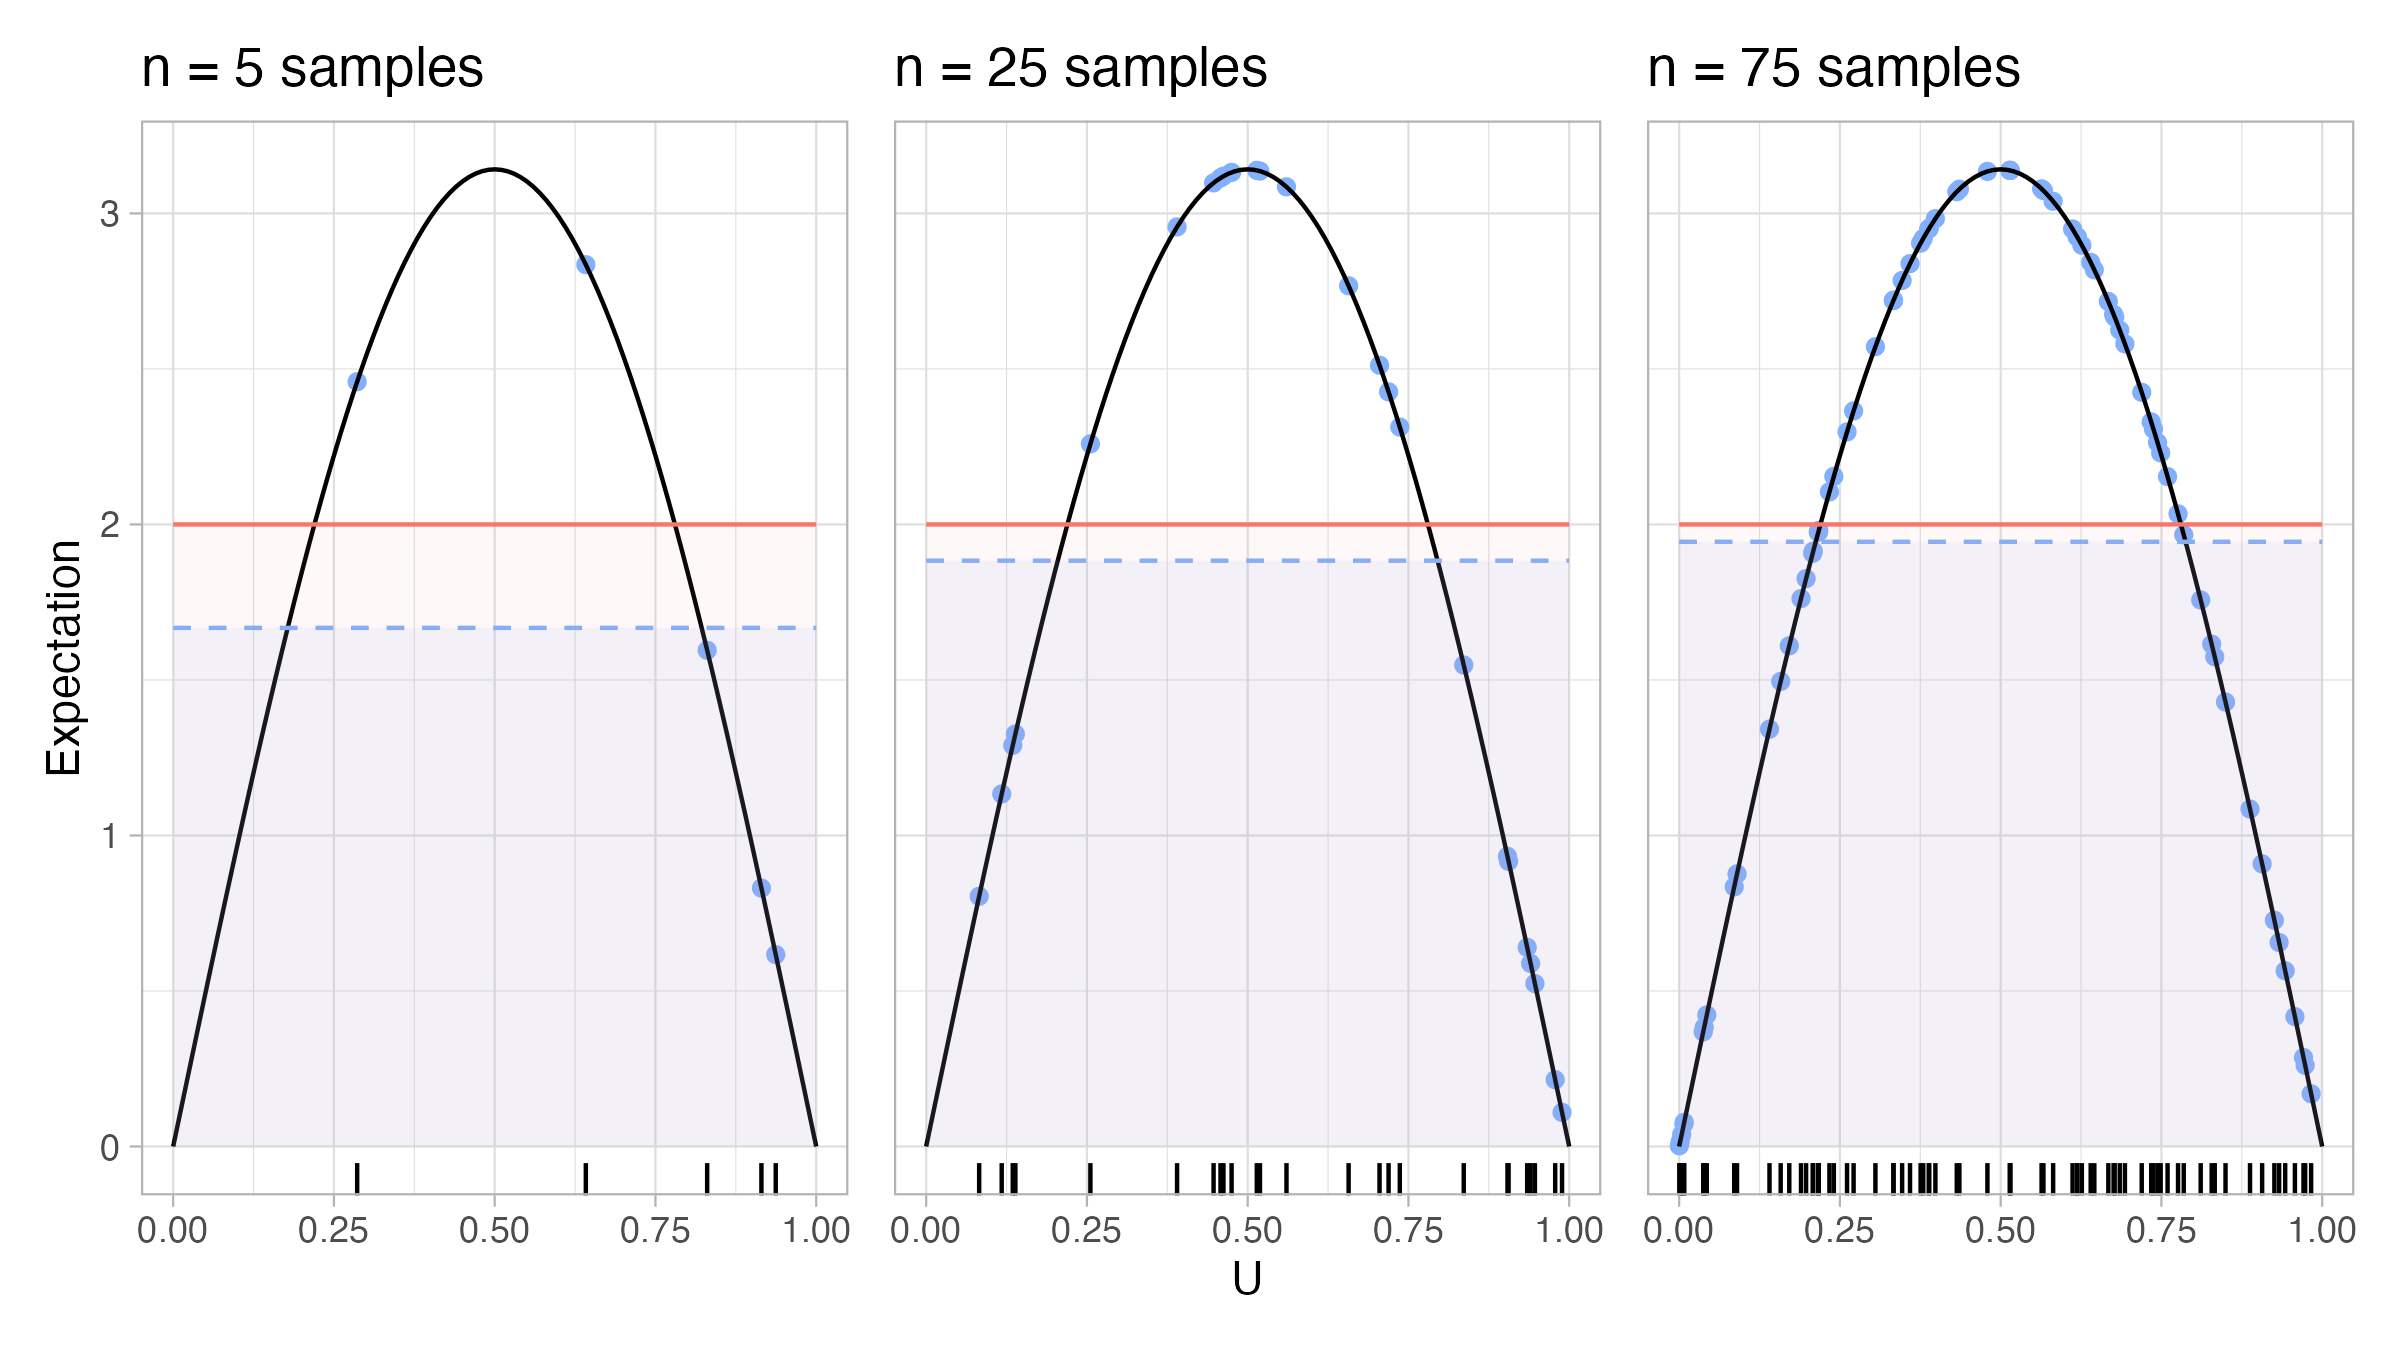
\includegraphics[width=.8\linewidth]{figures/mc-integration1.png}
    \caption{Monte Carlo approximation of $\int_0^{\pi} \sin(x)\,dx$ showing convergence to the true value of 2 as sample size increases. Generated using \href{https://github.com/NikoGerman/Seminar/blob/main/Notebooks/mc-integration.Rmd}{\texttt{mc-integration.Rmd}}.}
    \label{fig:mc-integration1}
\end{figure}
\end{example}

A comprehensive analysis of example \ref{ex:sin}, including convergence behavior and implementation details, can be found at \href{https://nikogerman.github.io/Seminar/Notebooks/mc-integration.html}{\texttt{mc-integration.html}}.

\subsection{Numerical integration and the curse of dimensionality}
An alternative to Monte Carlo integration is numerical integration, where traditional quadrature methods evaluate the integrand at regularly spaced grid points. While effective for low-dimensional problems, these methods suffer from the curse of dimensionality.
Maintaining accuracy requires $\tilde{N} = N^d$ function evaluations, where $N$ is the number of points per dimension and $d$ is the dimensionality. For example, a three-dimensional problem with $N=100$ points per dimension requires $100^3 = 10^6$ evaluations. Moreover, for the trapezoidal rule, the approximation error scales as $\mathcal{O}(\tilde{N}^{-2/d})$, making convergence prohibitively slow in high dimensions.
\begin{example}
\label{ex-cod}
Consider the $d$-dimensional integral
$$
\int_{[0,1]^d} f(\mathbf{x}) d\mathbf{x}
$$
where $f(\mathbf{x}) = 1$ if $x_i\in [0.4,0.6]$ for all $i=1,\dots,d$ and $f(\mathbf{x}) = 0$ otherwise.
Only $[0.2]^d$ of grid points contribute to the integral: 4\% for $d=2$, 0.032\% for $d = 5$, and less than $10^{-7}$\% for $d = 10$.
\end{example}
This \textit{curse of dimensionality} makes Monte Carlo methods particularly attractive, as their error depends only on $N$, not on dimensionality.

\subsection{Properties of the Monte Carlo Estimator}
The Monte Carlo estimator approximates the true expectation $\mu = \mathbb{E}_f[\varphi(X)]$ by averaging the function values $\varphi(X_i)$ over $n$ independent samples from the distribution $f$.

\begin{lemma}
\label{lemma-measurable-composition}
If $\varphi$ is a measurable function and $X_1, \ldots, X_n$ are i.i.d. random variables, then $\varphi(X_1), \ldots, \varphi(X_n)$ are also i.i.d. random variables.
\end{lemma}

\begin{proof}
This follows from the fact that the composition of a measurable function with a random variable is a random variable, and independence is preserved under measurable transformations.
\end{proof}

\begin{theoremrep}[Unbiasedness]
\label{theorem-unbiased}
The Monte Carlo estimator $\hat{\mu}_n$ is unbiased: 
\begin{equation}
    \mathbb{E}[\hat{\mu}_n] = \mu
\end{equation}
\end{theoremrep}

\begin{proof}
Assume $\mathbb{E}_f[\varphi(X)] = \mu$ exists. Then:
\begin{align*}
\mathbb{E}[\hat{\mu}_n] &= \mathbb{E}\left[\frac{1}{n}\sum_{i=1}^n\varphi(X_i)\right] \\
&= \frac{1}{n}\sum_{i=1}^n\mathbb{E}[\varphi(X_i)] \quad \text{(linearity of expectation)} \\
&= \frac{1}{n}\sum_{i=1}^n\mu \quad \text{(identical distribution)} \\
&= \mu
\end{align*}
\end{proof}

\begin{theoremrep}[Variance]
\label{theorem-variance}
The variance of the Monte Carlo estimator is 
\begin{equation}
    \text{Var}[\hat{\mu}_n] = \frac{\sigma^2}{n}
\end{equation}
where $\sigma^2 = \text{Var}_f[\varphi(X)]$.
\end{theoremrep}

\begin{proof}
Assume $\text{Var}_f[\varphi(X)] = \sigma^2 < \infty$. Then:
\begin{align*}
\text{Var}[\hat{\mu}_n] &= \text{Var}\left[\frac{1}{n}\sum_{i=1}^n\varphi(X_i)\right] \\
&= \frac{1}{n^2}\sum_{i=1}^n\text{Var}[\varphi(X_i)] \quad \text{(independence)} \\
&= \frac{1}{n^2} \cdot n \cdot \sigma^2 \quad \text{(identical distribution)} \\
&= \frac{\sigma^2}{n}
\end{align*}
\end{proof}

\begin{theorem}[Asymptotic Normality]
\label{theorem-clt}
Under regularity conditions, the Monte Carlo estimator satisfies:
\begin{equation}
\hat{\mu}_n - \mu \xrightarrow{d} \frac{1}{\sqrt{n}}\mathcal{N}(0, \sigma^2)
\end{equation}
\end{theorem}

This follows from the Central Limit Theorem\footnote{see Appendix \ref{appendix:clt}}. The key insight is that the estimation error decreases as $\mathcal{O}(n^{-1/2})$, independent of the dimension $d$ of the integration domain. This is the fundamental advantage of Monte Carlo methods over grid-based integration approaches in high-dimensional settings. Figure \ref{fig:mc-integration2} illustrates this convergence behavior by showing the estimation error for the integral from example \ref{ex:sin}.
\begin{figure}[h]
    \centering
    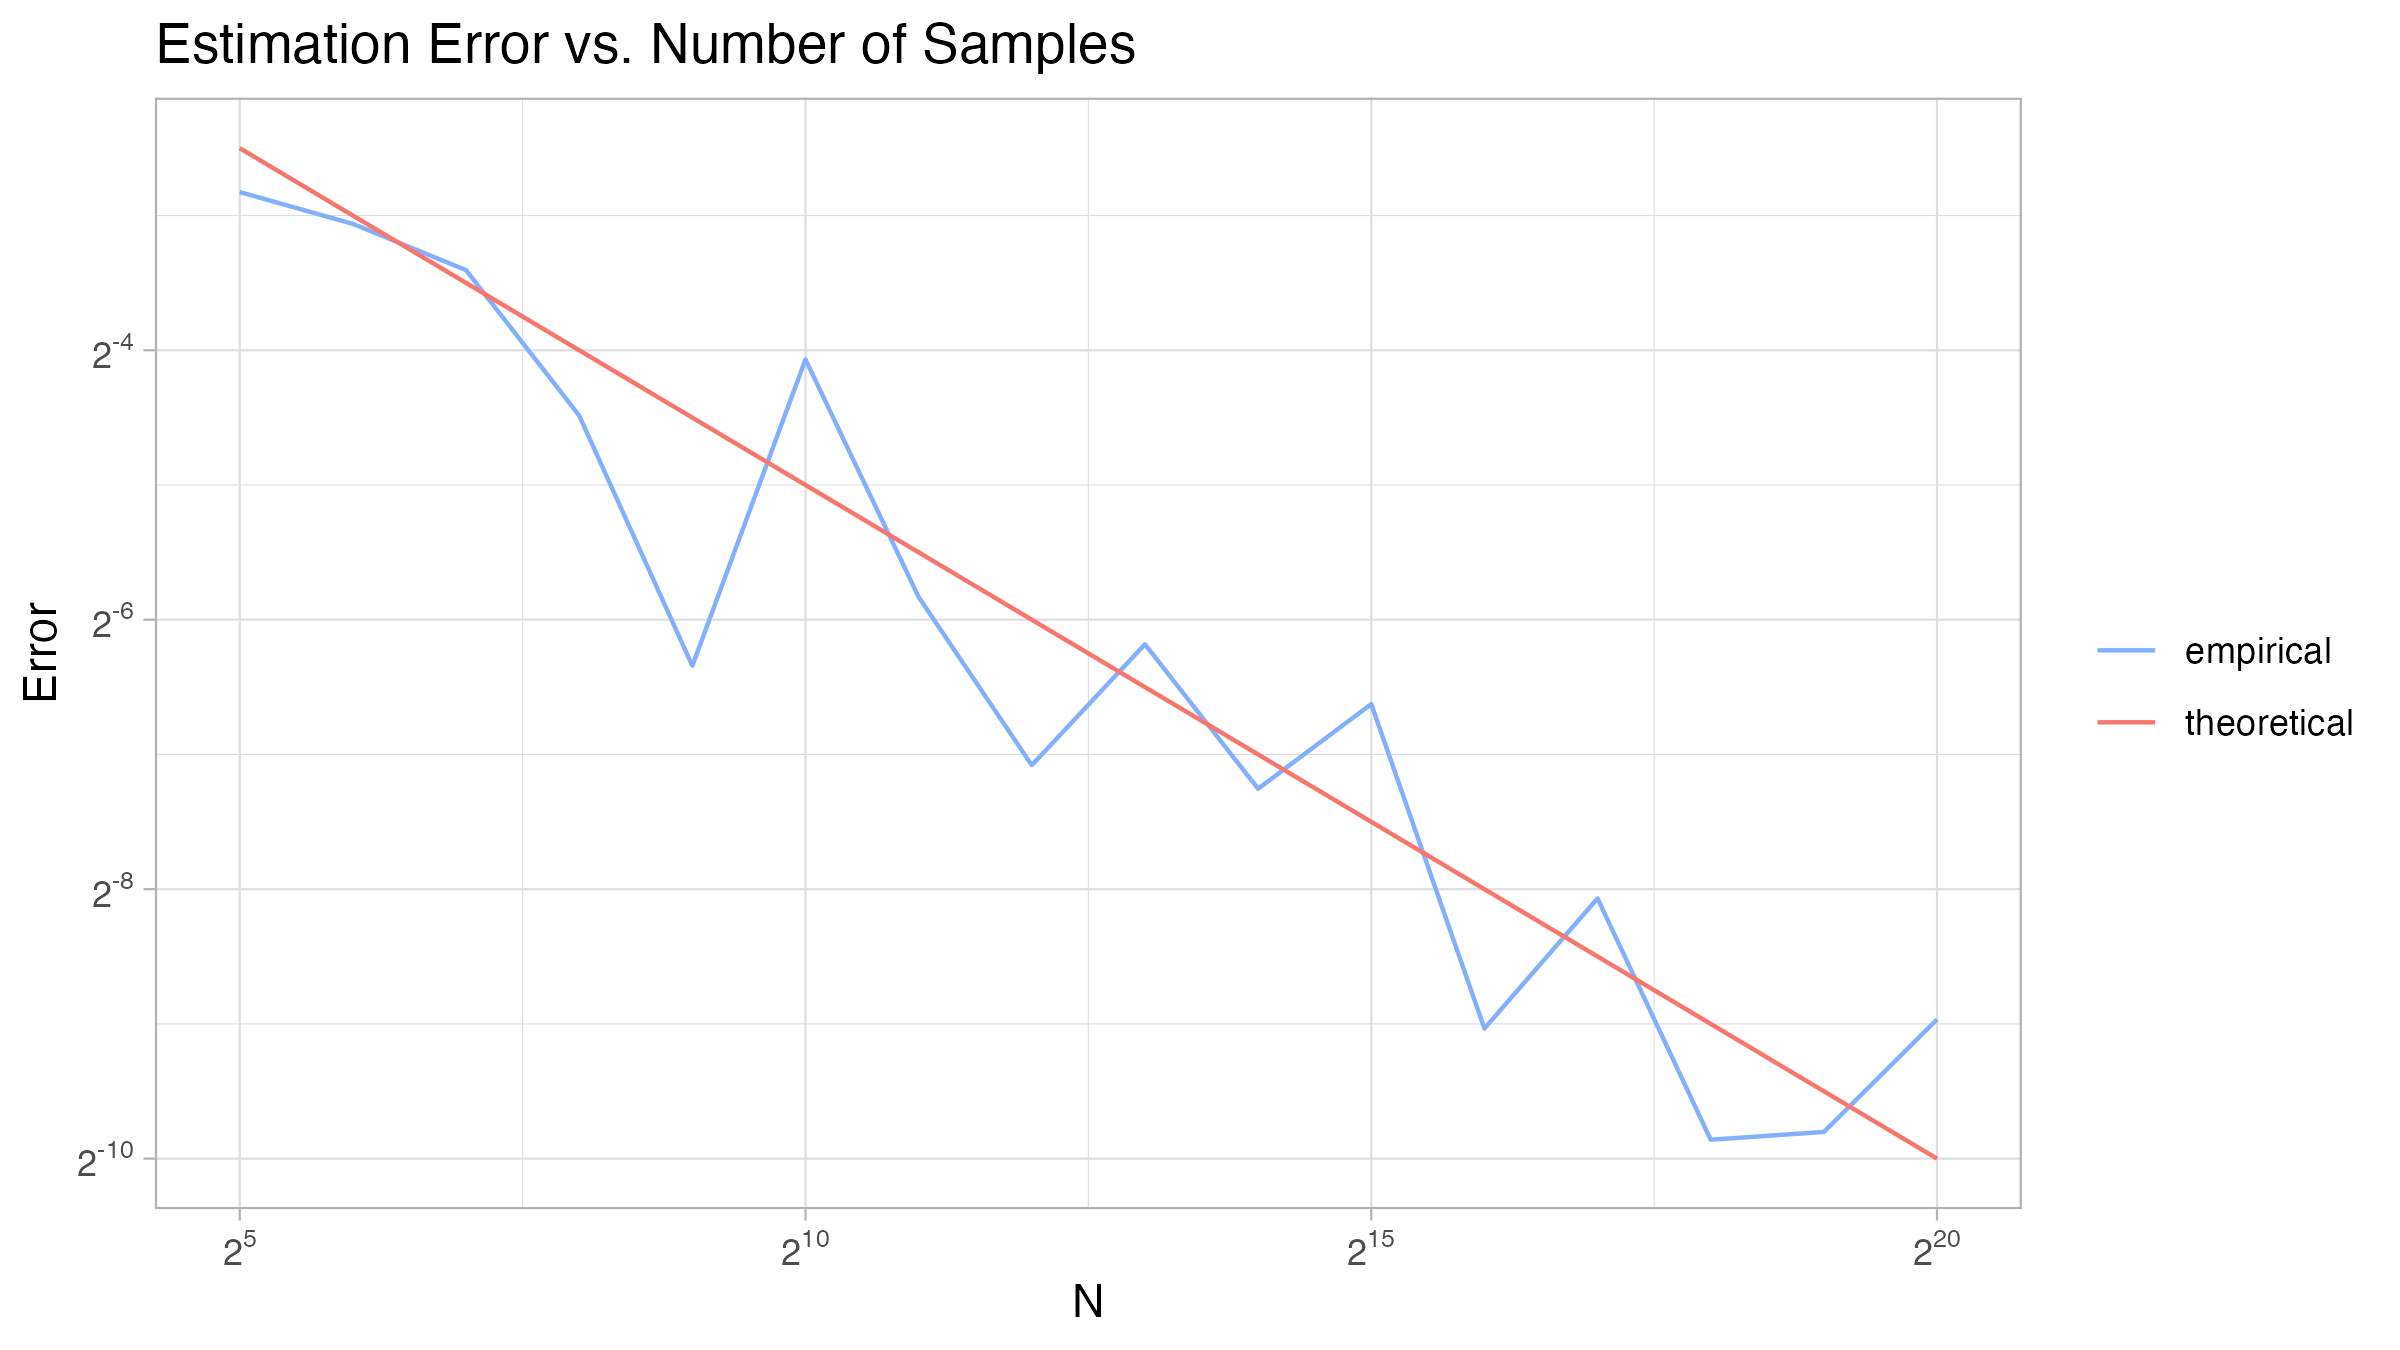
\includegraphics[width=.8\linewidth]{figures/mc-integration2.png}
    \caption{Estimation error for Monte Carlo approximation of $\int_0^{\pi} \sin(x)\,dx$ demonstrating the $\mathcal{O}(n^{-1/2})$ convergence rate. Generated using \href{https://github.com/NikoGerman/Seminar/blob/main/Notebooks/mc-integration.Rmd}{\texttt{mc-integration.Rmd}}.}
    \label{fig:mc-integration2}
\end{figure}


\paragraph{Confidence Intervals}
The asymptotic normality result from Theorem \ref{theorem-clt} enables the construction of confidence intervals for Monte Carlo estimates. 

Since $(\hat{\mu}_n - \mu) \xrightarrow{d} \frac{1}{\sqrt{n}}\mathcal{N}(0, \sigma^2)$, we can approximate the distribution of $\hat{\mu}_n$ as $\mathcal{N}(\mu, \sigma^2/n)$ for large $n$. In practice, the unknown variance $\sigma^2$ is estimated by the sample variance:
\begin{equation}
\hat{\sigma}^2_n = \frac{1}{n-1}\sum_{i=1}^n(\varphi(X_i) - \hat{\mu}_n)^2
\end{equation}
An approximate $(1-\alpha)$-confidence interval for $\mu$ is then given by:
\begin{equation}
\hat{\mu}_n \pm z_{\alpha/2} \frac{\hat{\sigma}_n}{\sqrt{n}}
\end{equation}
where $z_{\alpha/2}$ is the $(1-\alpha/2)$-quantile of the standard normal distribution. This interval provides a measure of uncertainty in the Monte Carlo estimate, with the width decreasing proportionally to $n^{-1/2}$ as the sample size increases.